\chapter{RFX-Hunch: a closed example based on electron temperature}
\label{section:RFXhunch}

With the aim at selecting an informative example of plasma computation that the machine learning could be devoted to, we chose to look at the temperature profiles that are coming from the Soft X-Ray diagnostics at RFX. The particular choice had been mainly motivated by the fact that it provides an example that can be a good representative factor of the plasma global configuration, being at the same time not too complex to be handled by simple networks. The electron temperature profile represents indeed a very important clue for looking at the plasma state that is very often accessed by physicists during analysis: it can be seen as an instant property that is almost ergodic during the pulse, it is acquired with a good temporal resolution, and that can be related to the magnetic configuration for the chosen time sample.

A plasma is composed with a mixture of species characterized by their own mass and electric charge. As first approximation, the plasma may be considered as consisting of two fluids mixed together: the first composed by the electrons and the second by the ions, or to be more specific by all the other heavy species: ions, neutral atoms, and other compound molecules.

What matters for a fusion machine is actually the ions temperature because electrons are not directly involved on fusion process.
Nevertheless electrons acquire energy from the electric field, which energizes the plasma, and lose part of it through elastic or inelastic collisions; in this way the plasma can move energy from one fluid to the other. For this reason in \textit{Tokamaks} this represents a direct handle for plasma heating through \acs{ECRH} plants. In RFX we don't have such input and the electron temperature are almost directly related to the plasma current and the magnetic pressure (\textit{pinch} effect).
In addition the acquired profile represents a local information of the internal state of plasma giving a chance to see through the simple external configuration.
\begin{figure}
    \centering
    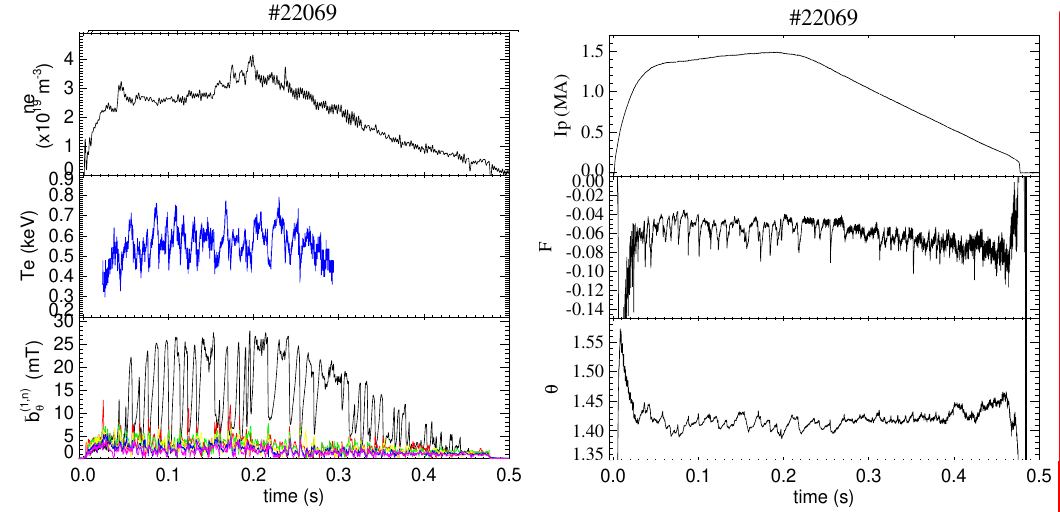
\includegraphics[height=5cm]{img/rfx/shot_example.png}
    \caption{Caption}
    \label{fig:rfx_shot_22069}
\end{figure}
This holds for the Thomson scattering too, indeed: the SXR invese-transformed profile of the plasma bremsstrahlung radiation, and the intensity of the scattered light from TS, provide the same kind of measure being both of them related to electrons velocity.
However, as already discussed, the two diagnostics are not interchangeable as they present different characteristics. In particular the TS is known to provide a more accurate measure both in spatial resolution and in the accuracy of the acquired quantity; on the other hand the SXR measure even being quite noisy, easily biased by plasma-wall interaction debris of carbon and other materials, and usually presenting a set of reconstructed points that vary in position and in number, has a very fine grained resolution in the time domain.
In RFX we have the SXR3 time resolution of about $500 \mu s$
\begin{figure}
    \centering
    \subfigure[]{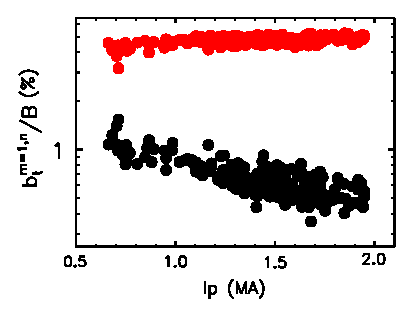
\includegraphics[height=3.8cm]{img/rfx/b7_bsec_ip.eps} \label{fig:rfx_parameters_a}}
    \subfigure[]{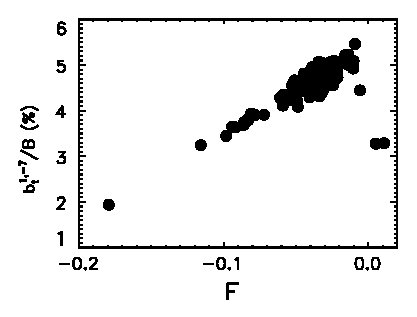
\includegraphics[height=3.8cm]{img/rfx/b7B_f.eps} \label{fig:rfx_parameters_b}}
    \subfigure[]{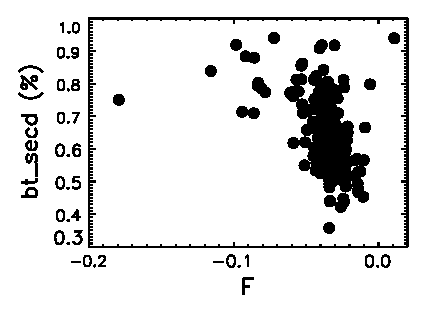
\includegraphics[height=3.8cm]{img/rfx/bsecB_f.eps} \label{fig:rfx_parameters_c}}
    \subfigure[]{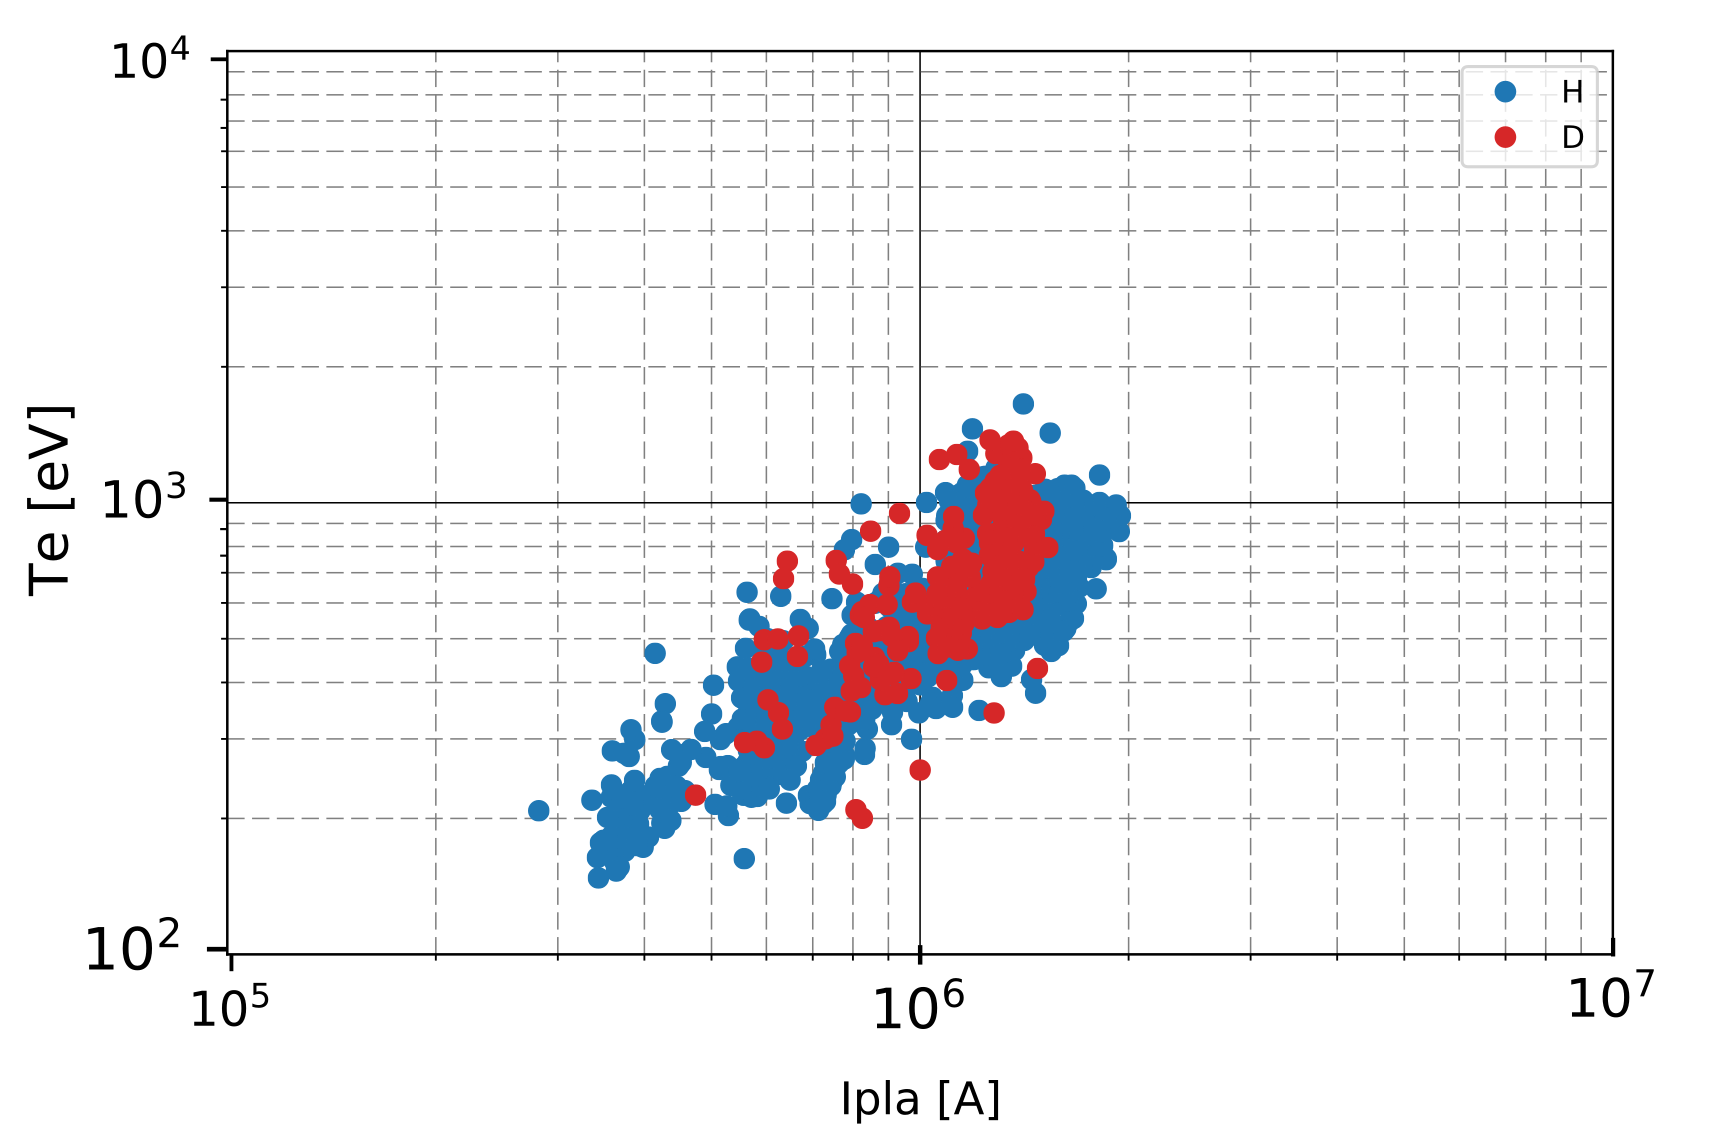
\includegraphics[height=4cm]{img/rfx/te_ipla.png} \label{fig:rfx_parameters_d}}
    \caption{Some plasma parameters correlation scatter plots from RFX-mod RFP experimental campaigns, respectively: the dominant mode (red markers) and secondaries (black markers) vs the plasma current $I_p$ (a), the dominant, and the secondaries vs the reversal parameter (b,c), and the mean plasm electron temperature $T_e$ vs the plasma current (d). }
    \label{fig:rfx_parameters}
\end{figure}


%  ____        _                 _   
% |  _ \  __ _| |_ __ _ ___  ___| |_ 
% | | | |/ _` | __/ _` / __|/ _ \ __|
% | |_| | (_| | || (_| \__ \  __/ |_ 
% |____/ \__,_|\__\__,_|___/\___|\__|
                                   
\section{Constructing the dataset} % SHAx

Once selected the set of signals that were thought to present all needed ingredient for reconstructing the plasma configuration a complete dataset able to comply with \Tensorflow input data of the fitting algorithms. Within the \acs{TF} framework a particular structure is devoted to represent such dataset; this structure is meant to provide a set of commodity routines that are used afterwards to handle the training process organization, such as: the split of training and validation data, the batching subdivision, the mapping for adapting to the particular model, applying data regularization algorithm (simple shuffling for example), and so forth.
For this reason making out fusion data compatible with this structure is a key point to have a flexible input for all possible constructed network and ML models. 
This structure is defined in a special \TF object class that can be simply included in python source directly reading a sequence array, a record array of structured data, or even a \Pandas \textit{dataframe}.

Although this is the actual structural output shape of our dataset we had to cope with the heterogeneity of our data sources: being part of the signal dataset coming from a \IDL data-structure array of a complex and accurate selection on relevant experiment pulses~\cite{Gobbin_QSH}, and part from raw or elaborated signals directly read from the global \MDSplus database of pulses.
For this reason we chose to make a first collection of all signal in a separate database that could be thought as a signal common cache of all the used components in the presented ML recipes.
This dataset represents also a further useful mean of data handling, being provided with tools such as: ordered or normalized subsets generator, or interactively selection of the missing data representative symbol (i.e. NaN flavors, zero float, negative sign, etc.).
Moreover an interactive collating signal selector has been implemented that can generate sets of arrays of signals data composed by sequence of inputs selected by name. In this way we could have a direct array of parameters by a simple query: for example with the string "\texttt{t\_Ip\_Vt\_Theta\_F}" the output would be a list of all times in all pulses made by arrays with [\textit{time}, \textit{plasma current}, \textit{toroidal loop voltage}, \textit{theta parameter}, \textit{reversal parameter}].

After the definition of the data the target \TF dataset adaptation has been done using the dedicated \TF \verb|Dataset.dataset_from_generator()| function. This is particularly useful because it can dynamically adapt to the particular input, and will be the suitable tool for the future enhancement to any possible dynamic source selection (i.e. the direct \MDSplus query or any other).
In the following a related code has been extrapolated from our dataset definition:
%
\begin{lstlisting}[language=Python, caption=Dataset from generator]
    def tf_tuple_compose(self, fields=[]):
        def clip(x):
            try: 
                if len(x) > self.dim: x=x[0:self.dim]
            except: pass
            return x
        def gen():
            import itertools
            for i in itertools.count(0):
                if i < len(self):
                    qsh = self[i]
                    yield tuple([ clip(qsh[n]) for n in fields])
                else:
                    return

        d0 = tuple([ clip(self[0][n]) for n in fields])
        types = tuple([tf.convert_to_tensor(x).dtype for x in d0])
        shape = tuple([np.shape(x) for x in d0])
        return tf.data.Dataset.from_generator(gen, types, shape)
\end{lstlisting}
%
here the generator function is the nested defined method called \verb|gen()| that yields the dataset components from a itertool object or simply return if we ran out of dataset bounds. The last is the defined identification of the sequence termination\footnote{this is not actually a mandatory behavior, we could have a function that generates new unseen data \textit{ad libitum} without haveing to cope with validation restrains or shuffling batches}.
Afterwards the extracted datum is packed in a \TF input tensor specifying tuples of its type and shape.

The final dataset was eventually composed by a list of arguments chosen from the list in~\Table{\ref{tab:database}}.
In particular concerning the electron temperature we composed the \textbf{te} elements as the y-axis and either \textbf{prel} or \textbf{rho} for the x-axis of the profile. 
\begin{table}[]
    \centering
    \begin{tabular}{l|l|l|l}
\textbf{tag} & \textbf{dtype} & \textbf{shape} & \textbf{description} \\
\hline
\verb|label      | & S10        & 1         &   pulse label with p\_number and time                 \\
\verb|pulse      | & np.int32   & 1         &   MDSplus pulse number                                \\
\verb|start      | & np.int32   & 1         &   start time                       \\
\verb|i_qsh      | & np.int32   & 1         &   number index of QSH in trend                        \\
\verb|tbordo     | & f4         & 1         &   temperature at the plasma border                    \\
\verb|tcentro    | & f4         & 1         &   temperature at plasma center                        \\
\verb|pos        | & f4         & 1         &   position of the maximum gradinet                    \\
\verb|grad       | & f4         & 1         &   estimated maximum gradient                          \\
\verb|n_ok       | & np.int32   & 1         &   number of valid temperature times in trend          \\
\verb|prel       | & f4         & (20,)     &   relative positions of the temperature profile       \\
\verb|rho        | & f4         & (20,)     &   remapped position of the temperature profile        \\
\verb|te         | & f4         & (20,)     &   acquired temperatures                               \\
\verb|Ip         | & f4         & 1         &   plasma current                                      \\
\verb|dens       | & f4         & 1         &   plasma density                                      \\
\verb|Te_dsxm    | & f4         & 1         &   temperature acquired by DSXM device                 \\
\verb|F          | & f4         & 1         &   reversal parameter                                  \\
\verb|TH         | & f4         & 1         &   theta striction parameter                           \\
\verb|POW        | & f4         & 1         &   Ohmic power released on plasma                      \\
\verb|VT         | & f4         & 1         &   loop toroidal voltage                               \\
\verb|VP         | & f4         & 1         &   loop poloidal voltage                               \\
\verb|B0         | & f4         & 1         &   root sum squared of the m=0 modes                   \\
\verb|B07        | & f4         & 1         &   amplitude of mode (0,-7)                            \\
\verb|B08        | & f4         & 1         &   amplitude of mode (1,-8)                            \\
\verb|B06        | & f4         & 1         &   amplitude of mode (1,-6)                            \\
\verb|B1         | & f4         & 1         &   root sum squared of the m=1 modes                   \\
\verb|B17        | & f4         & 1         &   amplitude of mode (0,-7)                            \\
\verb|B18        | & f4         & 1         &   amplitude of mode (0,-8)                            \\
\verb|B19        | & f4         & 1         &   amplitude of mode (0,-9)                            \\
\verb|NS         | & f4         & 1         &   dominant (1,-7) vs all the other m=1 modes          \\
\verb|mapro      | & f4         & (51,51)   &   reconstructed 2D map by SHEq code                   \\
\verb|xxg        | & f4         & (51,)     &   x-position grid for mapro                           \\
\verb|yyg        | & f4         & (51,)     &   y-position grid for mapro                           \\
\verb|n          | & i4         & (10,)     &   array of remapped modes                             \\
\verb|absBt_rm   | & f4         & (10,)     &   abs value for remapped $B_t$ at border              \\
\verb|argBt_rm   | & f4         & (10,)     &   arg value for remapped $B_t$ at border              \\
\verb|absBr_rm   | & f4         & (10,)     &   abs value for remapped $B_r$ at border              \\
\verb|argBr_rm   | & f4         & (10,)     &   arg value for remapped $B_r$ at border              \\
\verb|absFlux_rs | & f4         & (10,)     &   abs flux at resonance                               \\
\verb|argFlux_rs | & f4         & (10,)     &   arg flux at resonance                               \\
\verb|absBr_rs   | & f4         & (10,)     &   abs $B_r$ at resonance                              \\
\verb|argBr_rs   | & f4         & (10,)     &   arg $B_r$ at resonance                              \\
\verb|absBr_rp   | & f4         & (10,)     &   abs $B_r$ at plasma                                 \\
\verb|argBr_rp   | & f4         & (10,)     &   arg $B_r$ at plasma                                 \\
\verb|absBr_max  | & f4         & (10,)     &   abs $B_r$ maximum value                             \\
\verb|absFlux_max| & f4         & (10,)     &   abs flux maximum value
    \end{tabular}
    \caption{List of arguments for each element of the database where the input dataset is composed. }
    \label{tab:database}
\end{table}
From this point of view the generated signal can be seen just like the dummy example that has been used to investigate the properties of the variational autoencoder in section~\cref{section:VAE}; again we can see the variation on x-axis as an extension of the 1D signal to create a general function mapping in which the x-domain is the position on the direction of reconstructed measures and the y-domain is the related acquired temperature.
Beside the values of the actual y-axis temperature, the main difference from the previous generated dataset is that the related position, although being in the same way an ordered set, is not completely random, but the shift can be seen almost as an added structured noise.
This is in fact a slight simplification of the problem and for the model itself that relax the need of reconstructing the previously discussed \textit{elastic fit} factors in the latent space.
On the other hand what is reasonably to expect from those profile is a continuous passage from a flat low-temperature configuration to a central peaked curve where eventually the "\textit{hunch}" can be either centered or shifted depending on whether we are looking at a QSH or a MH configuration and also, in the former case, the actual poloidal position of the \textit{island} that directly depends on the phase of the running dominant mode.
It is nevertheless worth to be specified that both datasets, the dummy generated sum of gaussian envelops an the real temperature profiles, are formally identical in their public API. Therefore  any applied algorithm can be used with one or the other, with the same script structure; the main difference resides only in the supervised labelling: the real curves temperature profile does not provide the related associated label, that in the dummy case describes the generation class to which it belongs (previously named \textit{kind}).



%  __  __ _         _                   _       _        
% |  \/  (_)___ ___(_)_ __   __ _    __| | __ _| |_ __ _ 
% | |\/| | / __/ __| | '_ \ / _` |  / _` |/ _` | __/ _` |
% | |  | | \__ \__ \ | | | | (_| | | (_| | (_| | || (_| |
% |_|  |_|_|___/___/_|_| |_|\__, |  \__,_|\__,_|\__\__,_|
%                           |___/                        


%% FD-NT-27
\section{Handling missing data}

Within the input dataset, if any of \textbf{prel} or \textbf{rho} has been selected to describe the x-axis position on the electron temperature profile, it is almost immediate to see that the majority of samples is actually missing in some of the acquired position. This means that the number of real values for the corresponding line of sight have not been recorded. 
In the input dataset all arrays have been set to be left filled without spaces, from the minimum to the maximum x-position values, and a zero queue is left on the remaining. This is not acceptable to represent a valid network input as it would differently stimulate neurons with values that do not pertain to the same physical quantity, but are organized only by a favourable memory index.
A first reorganization was thus needed to define a set of new array position that are indexed on a the actual contained value basis.

The entire input array has been also defined over sized with respect to the complete acceptance of the actual positions. This means that the complete dataset could be reduced implementing a shrink of given set filling the gaps that have been left in these arrays. If all valid data - that account elements on the basis of a AND boolean operation between the non NULL data in x-position (either \textit{prel} or \textit{rho} arguments) and y-position (the Te temperature) - are reduced by sum along each element xy array, the overall distribution of the obtained sum values shows indeed a maximum of 18 counts, when the total size of each array is 20. Moreover, once the reordering of x-axis positions have been performed, and the zero populated elements removed, for some of the positions the NULL data persists again in almost the entire dataset (with very few exceptions). 

We finally decided to apply the reordering of the dataset x and y arrays using a k-means approach, defining the centroids on the basis of the x-value (i.e. the \textit{prel} position) on a total amount of $k=15$ clusters. This is actually a over constraint that loose some of the available information on the few input data that present more that 15 elements; however this allows to have a polluted set of positions to perform a useful training for all neurons that are facing the input features.
Another possible approach would have been to conversely apply a complete random position to the couple x-y leaving the network to perform a reordering on the firs layers; the casual selection on position is again needed to have a uniform population of input feature per neuron otherwise the training would expose an under-fitted set of weights on its internal kernel that would lead in turn to an undetermined local output on the network.
This refinement was not pursued at this first attempt though because we decided to maintain the overall needed network structure as simple as possible. In any event we leave it for a second stage of implementation to obtain a complete useful reconstruction of the profile.

That said, we are still facing a sparse input feature set where many values are NaN\footnote{NaN - litterally Not a Number - is a member of numeric data types to determine an undefined or unrepresentable value, especially in floating-point arithmetic. }. Unfortunately most generally available common implementations of neural network does not comply with NaN values. The common approach is to fill the empty gaps with a pre-computed value before the application to the neural network; this is commonly referred as \textit{data imputation} preconditioning. Many further approaches can be selected for this imputation algorithm, and a general accepted approach is a regression of some kind on the neighbour of missing data. This seemed a well documented and easy way to go at first glance; however in this dataset we are facing many adjacent missing data and a "simple" regression (polinomial or ridge) didn't produce a good fit for all the samples. 

Here comes the novel approach; as it has been already shown in~\cref{section:feedforward dense networks} we can see the network itself as a non linear regression operator, we could speculate that the network itself should be able to fill the gaps by means of available data, and it can also do this considering not only the single data under analysis, but the entire dataset.
Our very simple solution is sketched in~\Figure{\ref{fig:6_vae_missing}}
%
\begin{figure}
    \centering
    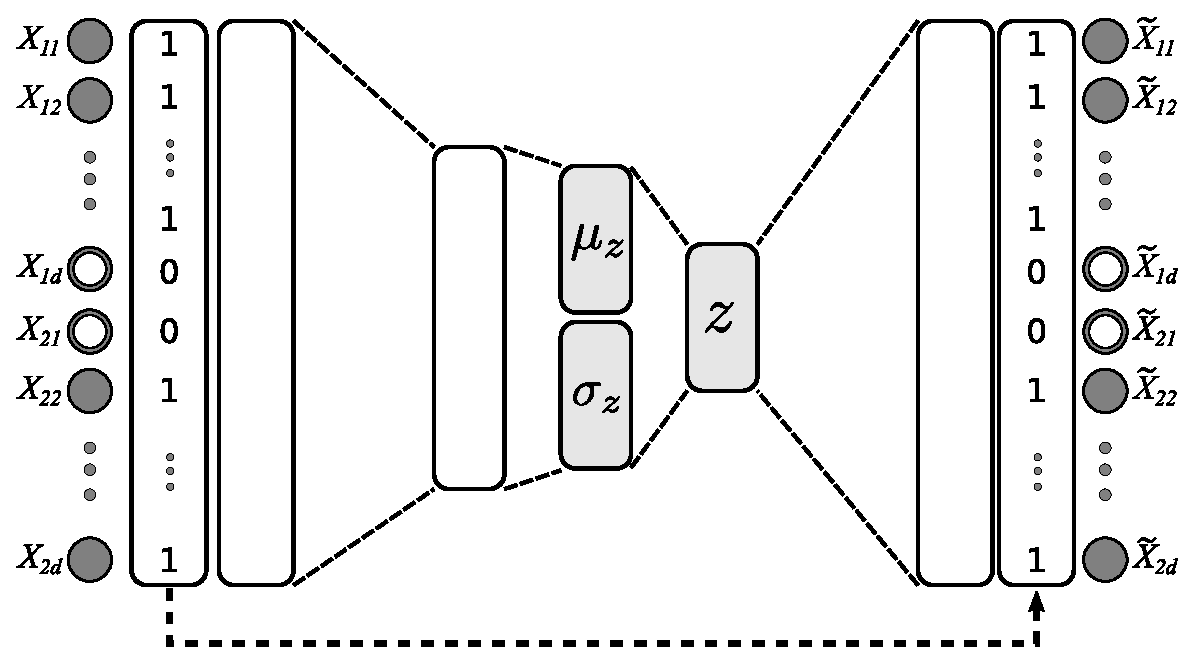
\includegraphics[height=6cm]{img/6_T_Hunch/VAE_MISSING.eps}
    \caption{VAE Missing point training NaN-Mask layer}
    \label{fig:6_vae_missing}
\end{figure}
%
where it can be seen that we applied the legacy \acs{VAE} schema with a sole couple of mirror layers added on the head and on the tail of the sample path through the network. In particular we added a simple input conditional layer, called \textbf{NaN-Mask} layer, that transforms all NaN to zero floats on the inference network, and at the same time the same mirrored transformation is applied on the network output erasing the generated network guess.
This is applied for all (and sole) training data; we chose to apply the zero float value to those inputs but any acceptable float would be equally accepted, because the magic is actually that the mirrored assignment on the output makes \textit{zero back-propagated error} for that input so the training simply does not see the missing data at all and proceed on training with the other available information.
\begin{figure}
    \centering
    \subfigure[]{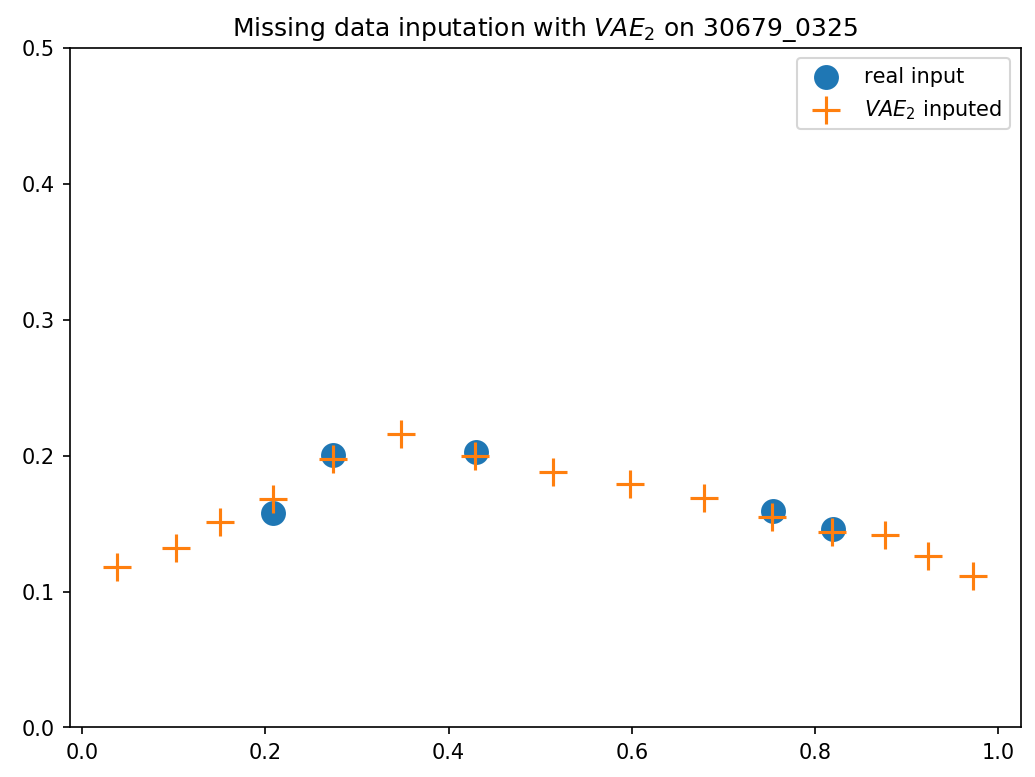
\includegraphics[width=4.8cm]{img/STEP7_CLEAN/missing_data_example.png}}
    \subfigure[]{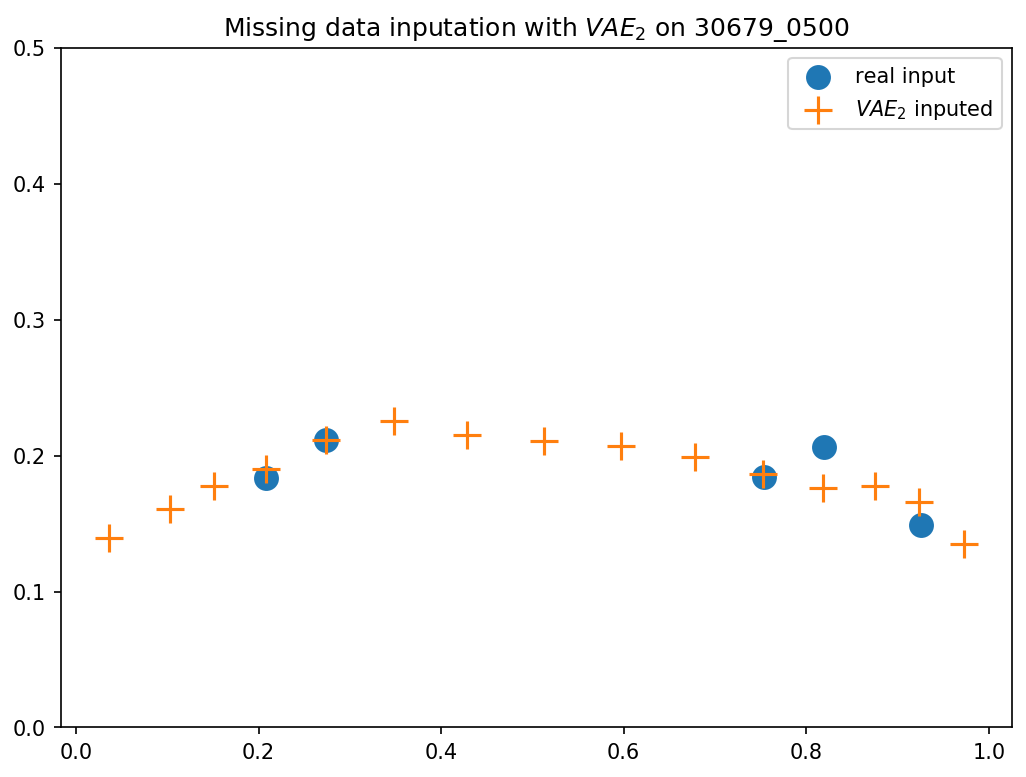
\includegraphics[width=4.8cm]{img/STEP7_CLEAN/missing_data_example2.png} \label{fig:missing data example_b}}
    \subfigure[]{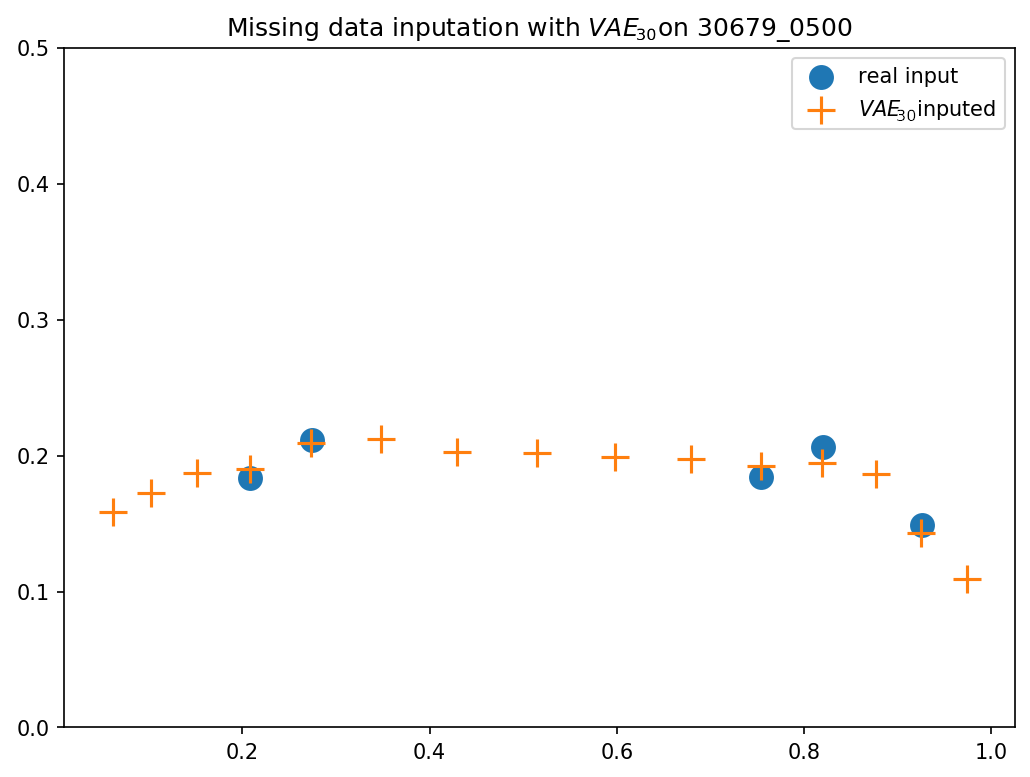
\includegraphics[width=4.8cm]{img/STEP7_CLEAN/missing_data_example3.png} \label{fig:missing data example_c}}
    \caption{Missing data example as seen by a simple generated output of \VAE{2} trained with NaN-Mask layers, where only 5 valid element were present in the input profile (a)(b); a slight effect of VAE denoising is also visible in (b) with VAE intrinsic smoothing overimposed, while the overcomplete recovery from \cref{section:recovery} has been applied on (c). }
    \label{fig:missing data example}
\end{figure}
Two examples of extreme missing data input have been proposed to a \VAE{2} model pre-trained with our NaN-Mask layers and are shown in~\Figure{\ref{fig:missing data example}}; on blue dots ($\bullet$) the input profile with missing points, and on red cross (+) the output of the network where the output mask layer is disabled guessing the profile form the reconstructed point in latent space.


%  ____                                    
% |  _ \ ___  ___ _____   _____ _ __ _   _ 
% | |_) / _ \/ __/ _ \ \ / / _ \ '__| | | |
% |  _ <  __/ (_| (_) \ V /  __/ |  | |_| |
% |_| \_\___|\___\___/ \_/ \___|_|   \__, |
%                                   |___/ 

\subsection{Data recovery and signal denoising}
\label{section:recovery}
In~\Figure{\ref{fig:missing data example}} an example of missing data recovery has been presented where a simple \VAE{2} model was able to generate the missing portion of the curve. The beauty of this imputing data approach, as already anticipated, is that the network proposes a regression that is based on available input data, but also on the complete dataset because it proposes an instance of a reconstructed space that comes form a likelihood maximized over the entire dataset.
However in~\Figure{\ref{fig:missing data example_b}} some points on the right side of the profile seem to be bad reconstructed, but this example was carefully selected to show on the contrary another concurrent effect of \acs{VAE} generative output: the data denoising.
This exploit the same principle that the reconstruction is treated scholastically, the effect is well known and fall into the category of \textbf{denoising autoencoders}.

To make autoencoder act as a denoiser the input is usually deliberately corrupted by randomly turning some of the features to zero. In general, the percentage of input nodes which are being zeroed is around 50\% but a lower count, such as 30\%, works as well; the actual optimal value seems almost depending on the amount of data and input nodes you have~\cite{ae_denoise}. In our case what we see is that the NaN-Mask is already doing that; we omitted to train the error on the NaN values as it drives the learning algorithm to a wrong bias, but the zeroed value just after the mask layer is seen by connected nodes just as a dropout would have been added to the network. So in this case we can say that the missing distribution is actually performing slight denoising of the input data; unfortunately this is not the sole component of the observed smoothing. If the added dropout helps the network to be more robust on input variation (denoising effect) on one side, it is also well known that VAE approach tends to add a slight blurring on the generated output~\cite{ghosh2019variational}. 

With the purpose of creating a network tailored for the electron temperature profile recovering we the \textit{recovery} method has been added to the VAE structure that follow the simple modification shown in~\Figure{\ref{fig:VAE_recovery}}.
As it can be seen from the schema the dual operation on masking NaN values is performed, where the mask remains active during training and than it is set to be always \textit{True} during recovery; it is also quite obvious that the generation network of the recovery operation takes its input from the mean values of the latent space, without performing the reparametrization (i.e. without applying any variational) because the space has been already shaped at this point.
%
\begin{figure}
    \centering
    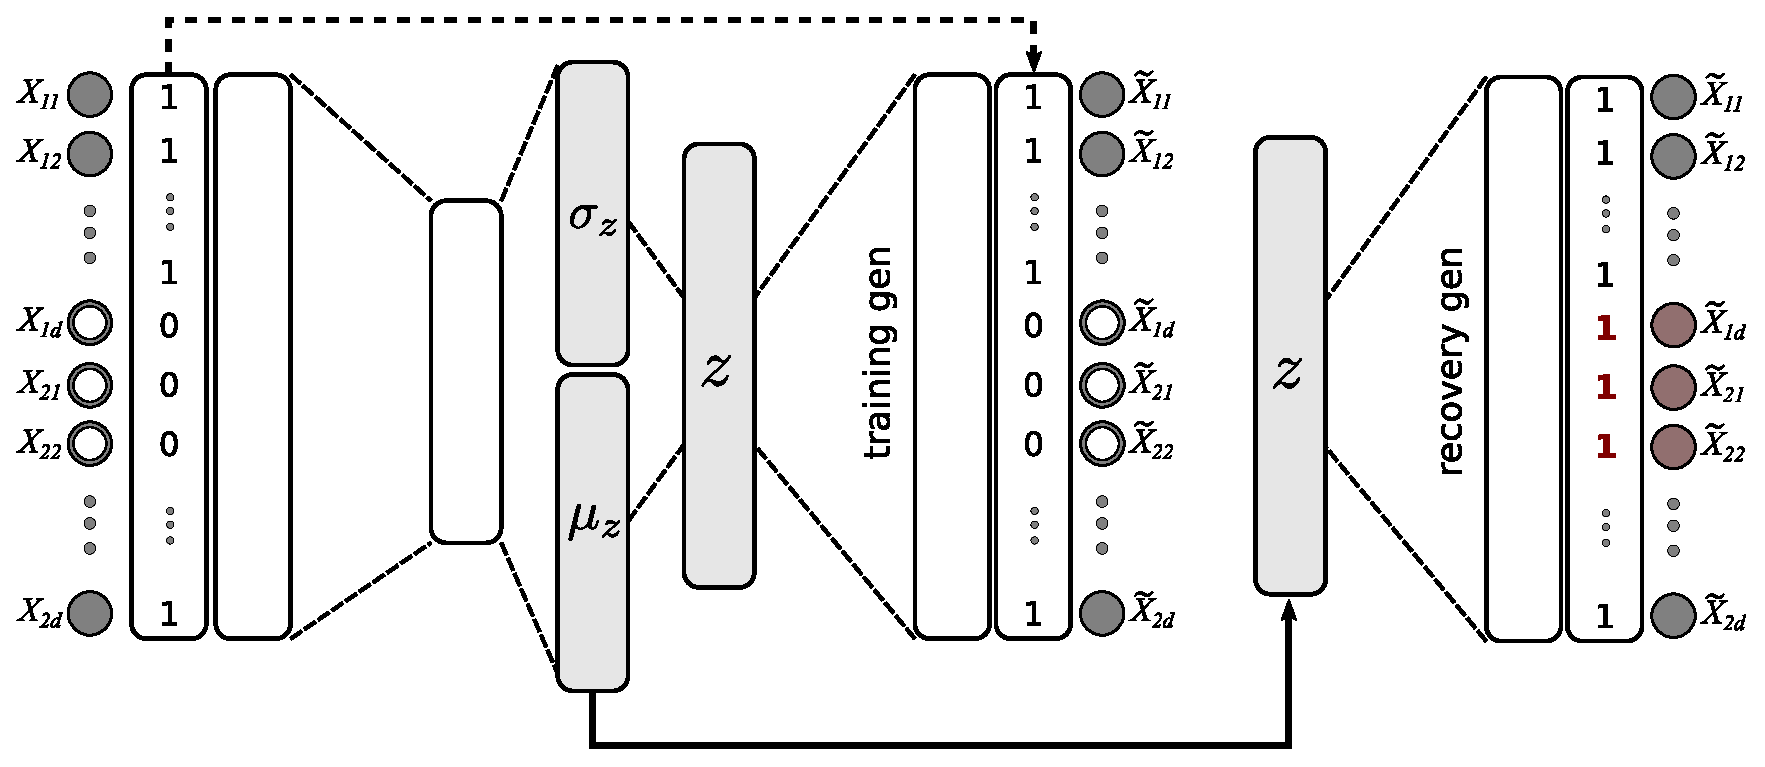
\includegraphics[height=6cm]{img/STEP7_CLEAN/VAE_CLEAN.eps}
    \caption{Recovery process of missing data}
    \label{fig:VAE_recovery}
\end{figure}
%
Our version of the recovery model structure is also \textit{overcomplete}: this means that the size of the latent space has its dimension size that equals or exceeds the size of the features dimension. Even if this condition could be thought as a possible loose of embedding properties for VAE, the final result shows to not fall on overfitting condition thanks to intrinsic self regulatory behavior~\cite{dai2017hidden}. We exploited this condition in recovery by setting the latent space with the same feature dimension; this has been represented in the same schema picture of~\Figure{\ref{fig:VAE_recovery}} by the enlarged size of the variational components ($\sigma_z, \mu_z, z$). This shown to reduce the blur effect over denoise, helping to provide a good fit on output recovered data vs missing features.


%   ___  ____  _   _ 
%  / _ \/ ___|| | | |
% | | | \___ \| |_| |
% | |_| |___) |  _  |
%  \__\_\____/|_| |_|

\subsection{QSH latent space representation}

As a very first attempt the data form the SXR, without recovery cleaning, has been fed into a \VAE{2} network to create a easy browsable latent space, hoping to see a clusterization over the QSH states.
With this purpose a \VAE{2} model has been set with the following parameters: \\
\verb| latent_dim=2, feature_dim=30, dprate=0, scale=1, geometry=[20,20,10,10]|. \\
All input have been normalized and the dataset has been cleaned from profiles with less that 5 valid points.
The reconstructed latent space has been plotted in~\Figure{\ref{fig:VAE2_qsh_ls}} by means of 1000 samples randomly selected from dataset that were passed through the inference net (aka. the encoder step of VAE).
\begin{figure}
    \centering
    \subfigure[]{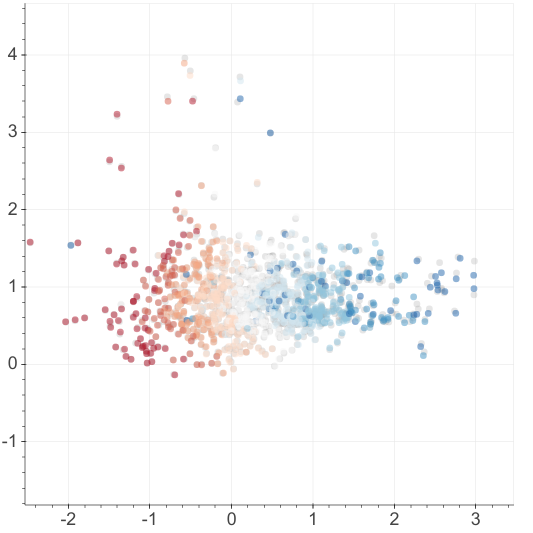
\includegraphics[height=4cm]{img/STEP7_CLEAN/ls2_tcentro.png} \label{fig:VAE2_qsh_ls_a}}
    \subfigure[]{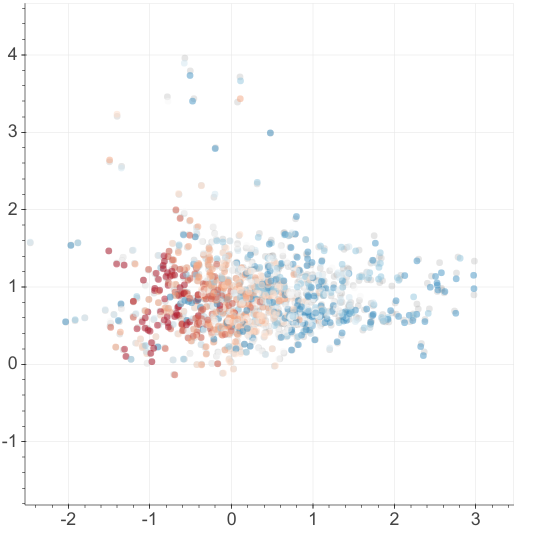
\includegraphics[height=4cm]{img/STEP7_CLEAN/ls2_tbordo.png} \label{fig:VAE2_qsh_ls_b}}
    \subfigure[]{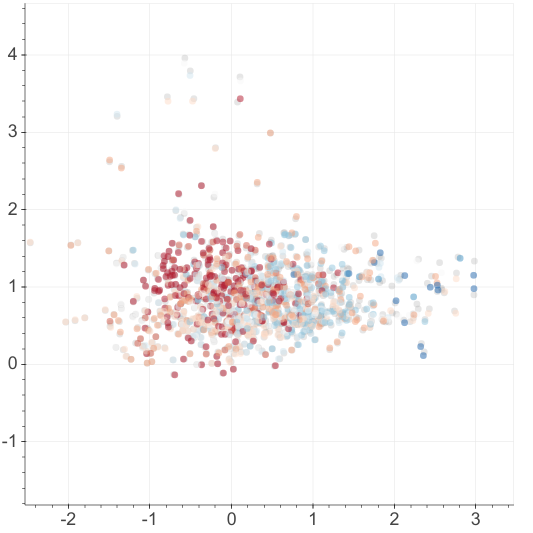
\includegraphics[height=4cm]{img/STEP7_CLEAN/ls2_Ip.png} \label{fig:VAE2_qsh_ls_c}}
    \caption{A scatter plot of 1K points representing a reconstructed \VAE{2} latent space where colour scale report external quantities respectively: the temperature $T_e$ at the center of plasma column (a), $T_e$ at border, and the plasma current $I_p$ for that pulse at that time. }
    \label{fig:VAE2_qsh_ls}
\end{figure}
The three plots shows the same latent distribution of given input with different chromatic tones: in the first and second pictures the normalized $T_e$ value at respectively the center and the border of plasma column has been represented by a tone scale that goes from blue to red at rising temperatures. In~\Figure{\ref{fig:VAE2_qsh_ls_c}} the external measure of plasma current has been also plotted with the same color scale to see the slight expected correlation between temperature and current.

As we chose to generate a simple 2-dimensional latent space it has been shown that the the representation in euclidean coordinates is trivial, and so it is to plot a point that can be fed in the generative network (aka. decoder set of VAE) too.
This helps to further discover how the latent space has been structured by the encoder; in figure~\Figure{\ref{fig:VAE2_qsh_gen}} five points have been selected and plotted on latent space (plots on the left), and the same have been decoded back to a guessed temperature profile (plots on right).
\begin{figure}
    \centering
    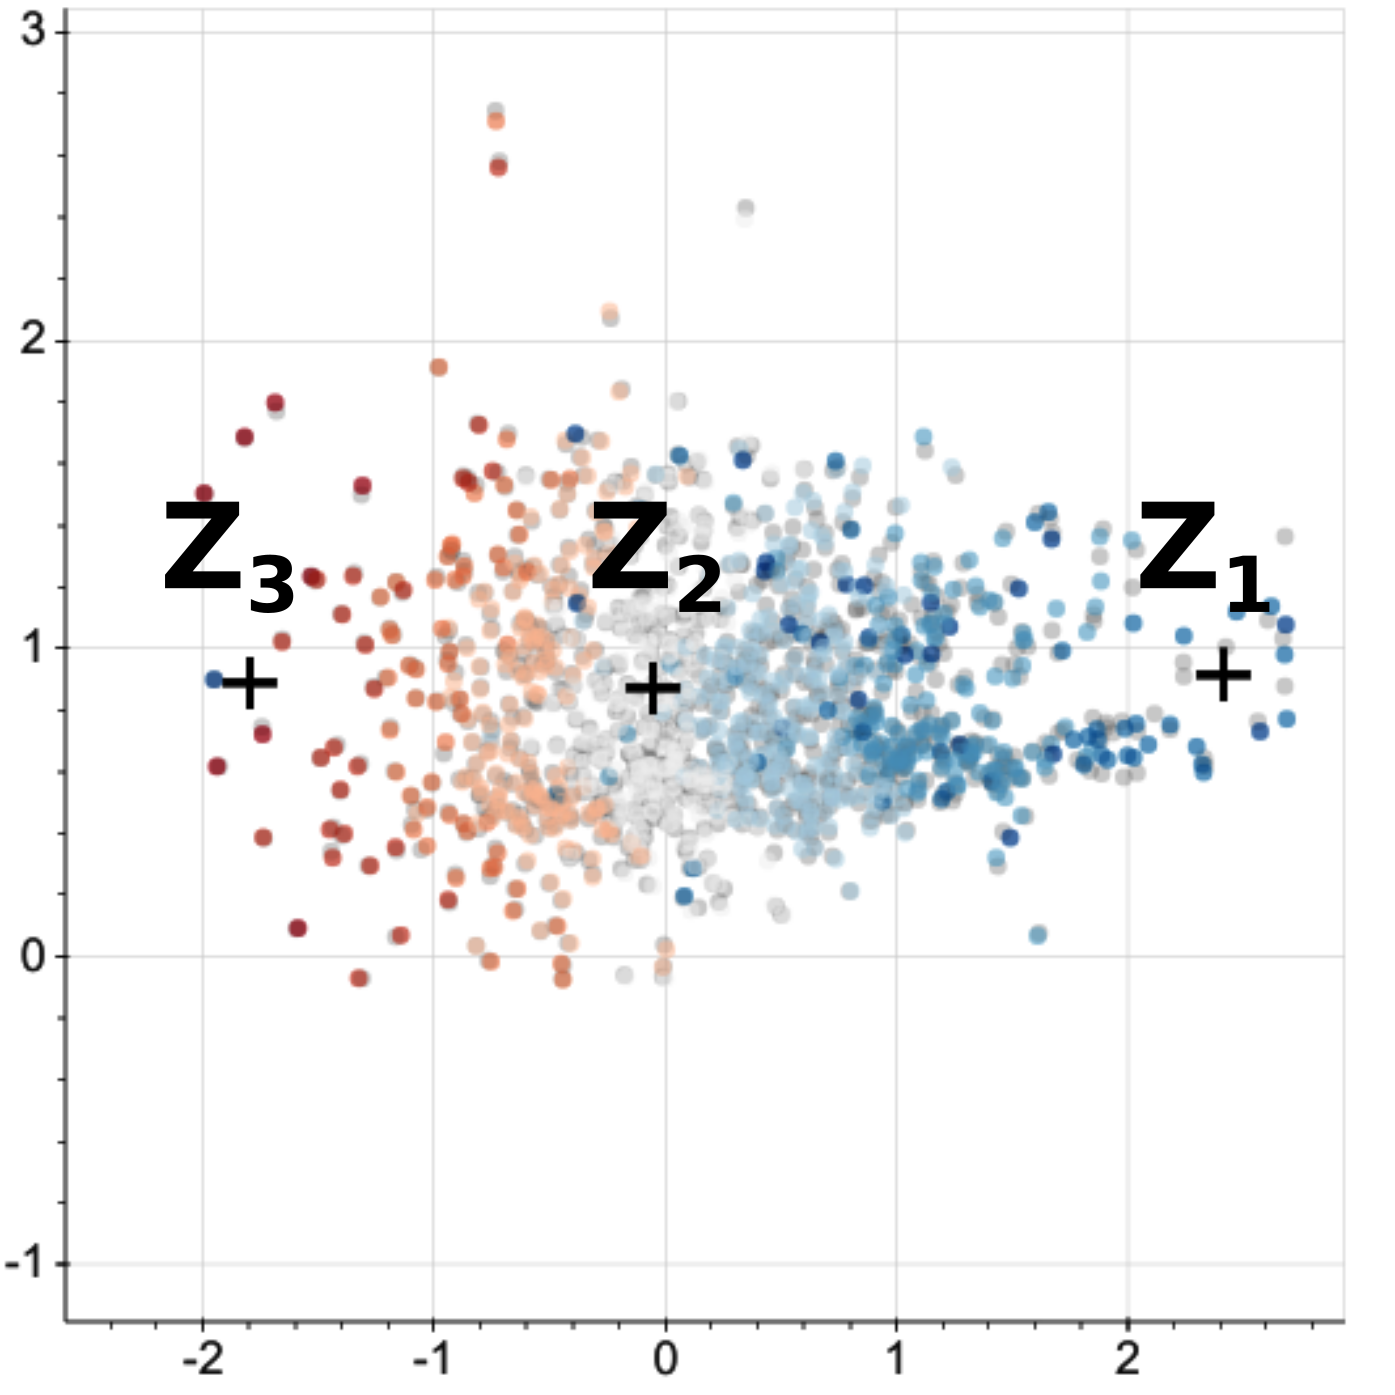
\includegraphics[height=4cm]{img/6_T_Hunch/ls_beta_tcentro_123.png}
    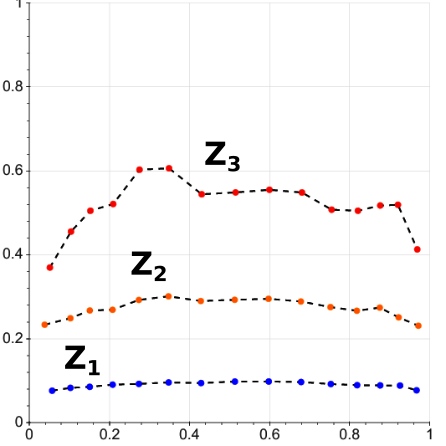
\includegraphics[height=4cm]{img/6_T_Hunch/ls_beta_tcentro_123_gen.png} \\
    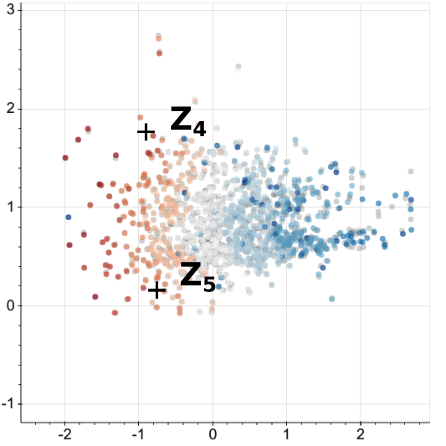
\includegraphics[height=4cm]{img/6_T_Hunch/ls_beta_tcentro_45.png}
    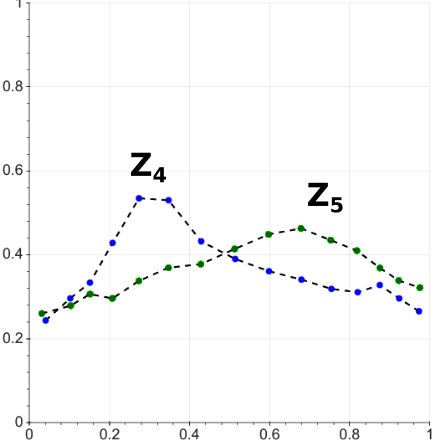
\includegraphics[height=4cm]{img/6_T_Hunch/ls_beta_tcentro_45_gen.png}
    \caption{Five profile curves generated by decoding the relative latent space points taken to characterize the main disentangled factor learnt by \VAE{2} on the entire $T_e$ dataset.}
    \label{fig:VAE2_qsh_gen}
\end{figure}
From the reconstructed curves it appears very clear that two different principal latent factors have been learnt: the former, shown by the progression ($z_1, z_2, z_3$), is the rising of the central temperature that well agree with the plotted color of $T_e$ at plasma center; the latter, shown by ($z_4, z_5$) is the two side extremes of the peak that correspond to the phase of the observed island.
It is also worth to note from the same figure the fact that the two possible factor that are represented in latent space have been aligned with the principal axes, an this proves a successful disentaglement of them made by the $\beta$-VAE application. 

The two factor that have been extracted by \VAE{2} are eventually quite trivial, and this come from the fact that we constrained the system to fit in two latent space dimensions. One could then try to use a preconditioning of the signal that remove one of the factor prior to the learning leaving that factor as a side fixed parameter that could be eventually applied at the generation output. This has been done for example in the same network removing the signal average that corresponds to the horizontal axis of the latent space.
The result is shown in~\Figure{\ref{fig:VAE2_qsh_ls_preconditioned}}
\begin{figure}
    \centering
    \subfigure[]{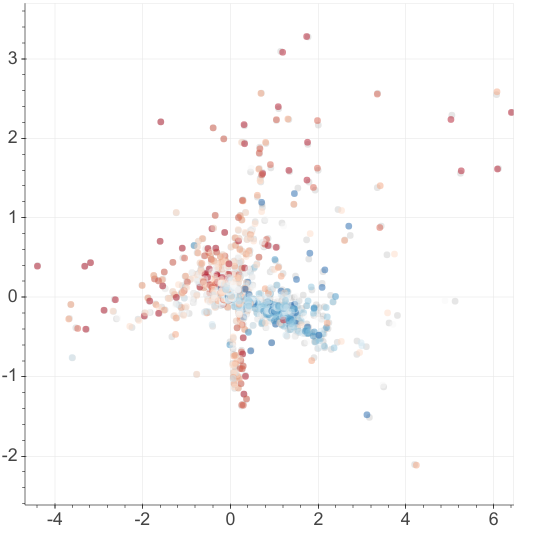
\includegraphics[height=5cm]{img/6_T_Hunch/ls_beta_clip_tcentro.png} \label{fig:VAE2_qsh_ls_preconditioned_a}}
    \subfigure[]{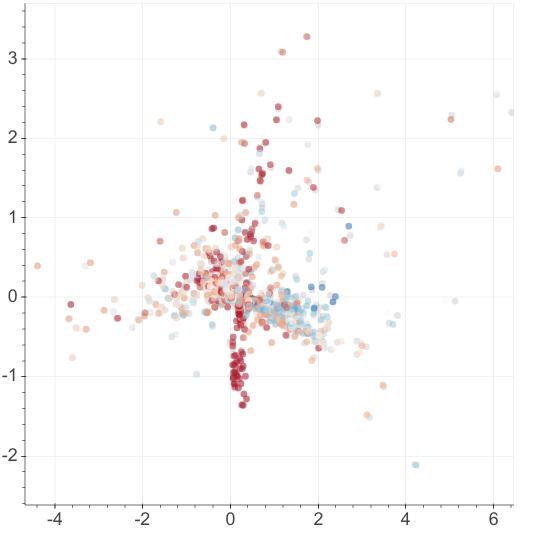
\includegraphics[height=5cm]{img/6_T_Hunch/ls_beta_clip_Ip.png} \label{fig:VAE2_qsh_ls_preconditioned_b}} \\
    \subfigure[]{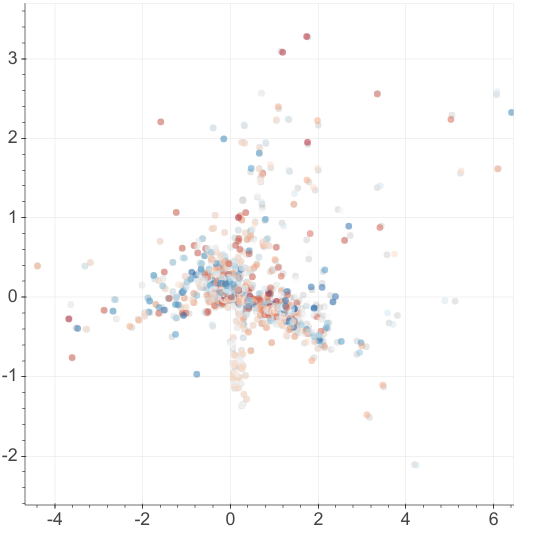
\includegraphics[height=5cm]{img/6_T_Hunch/ls_beta_clip_F.png} \label{fig:VAE2_qsh_ls_preconditioned_c}}
    \subfigure[]{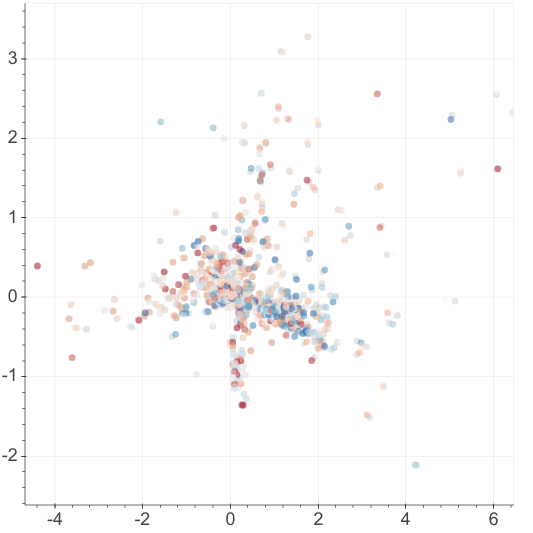
\includegraphics[height=5cm]{img/6_T_Hunch/ls_beta_clip_NS.png} \label{fig:VAE2_qsh_ls_preconditioned_d}}
    \caption{Latent representation of the normalized unbiased temperature profiles, where the color scale characterize respectively: the temperature at plasma center (a), the plasma current (b), the reversal parameter (c), and the dominant mode ratio (d).}
    \label{fig:VAE2_qsh_ls_preconditioned}
\end{figure}
In this case a more complex organization was captured; the four plots are representative of different external parameters, respectively: $t_e$ center, plasma current $I_p$, reversal parameter $F$, and the dominant perturbation vs all measured modes $NS$.
In \Figure{\ref{fig:VAE2_qsh_ls_preconditioned_b}} a marked vertical stripe of values sharing high plasma current is clearly visible overimposed to a more spread central cluster that rise in current from the right to the left. The central high current stripe is then further decomposed if we look at the center temperature in~\Figure{\ref{fig:VAE2_qsh_ls_preconditioned_a}}, while presents almost the same reversal parameter as in~\Figure{\ref{fig:VAE2_qsh_ls_preconditioned_c}}.

From the generative point of view the final profile behavior can be obtained form~\Figure{\ref{fig:VAE2_qsh_gen_prec_a}}: the central temperature has been represented as a anti-correlated function of the two latent variables ($z_1, z_2, z_3$) , while the QSH phase seems to be in the direct linear relation ($z_4,z_5$) as from~\Figure{\ref{fig:VAE2_qsh_gen_prec_b}}.
\begin{figure}
    \centering
    \subfigure[]{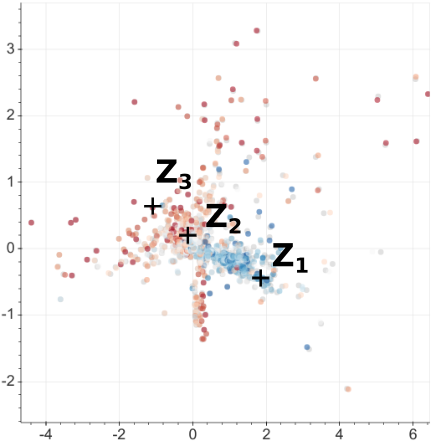
\includegraphics[height=4cm]{img/6_T_Hunch/ls_beta_clip_tcentro_123.png}  \label{fig:VAE2_qsh_gen_prec_a}}
    \subfigure[]{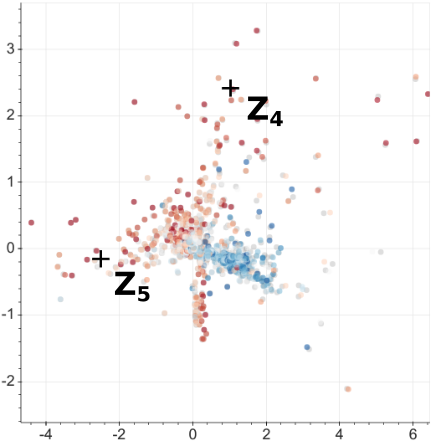
\includegraphics[height=4cm]{img/6_T_Hunch/ls_beta_clip_tcentro_45.png}  \label{fig:VAE2_qsh_gen_prec_b}}
    \subfigure[]{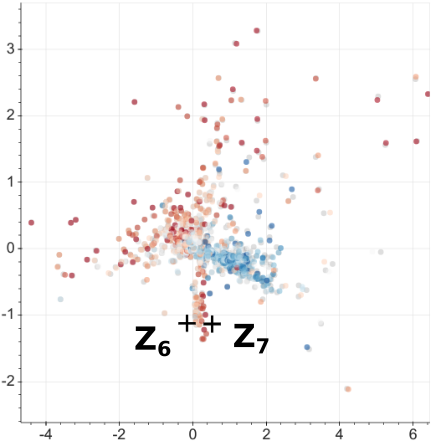
\includegraphics[height=4cm]{img/6_T_Hunch/ls_beta_clip_tcentro_67.png}  \label{fig:VAE2_qsh_gen_prec_c}}
    \subfigure[]{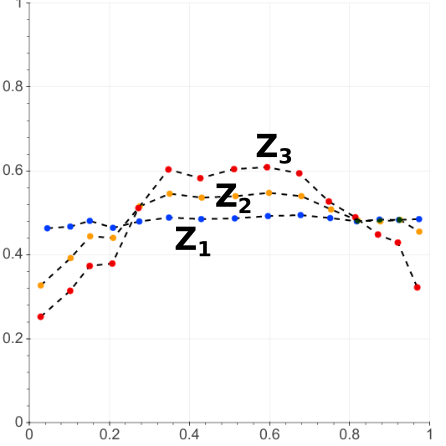
\includegraphics[height=4cm]{img/6_T_Hunch/ls_beta_clip_tcentro_123_g.png}  \label{fig:VAE2_qsh_gen_prec_d}}
    \subfigure[]{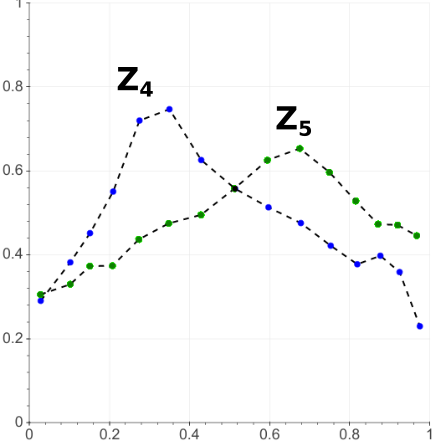
\includegraphics[height=4cm]{img/6_T_Hunch/ls_beta_clip_tcentro_45_g.png}  \label{fig:VAE2_qsh_gen_prec_e}}
    \subfigure[]{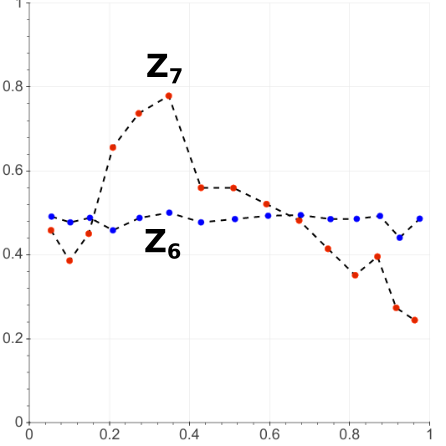
\includegraphics[height=4cm]{img/6_T_Hunch/ls_beta_clip_tcentro_67_g.png}  \label{fig:VAE2_qsh_gen_prec_f}}
    \caption{Seven profile curves generated by decoding the relative latent space points taken to characterize the the structure of the latent space in~\Figure{\ref{fig:VAE2_qsh_ls_preconditioned}} from a \VAE{2} trained with the normalized unbiased temperatures. }
    \label{fig:VAE2_qsh_gen_prec}
\end{figure}
The third profile has no trivial interpretation, even if the current and the reversal seems to be flat in that domain the temperature varies with a steep gradient along the minor dimension of the stripe, and proceeding along the rising temperature (from $z_6$ to $z_7$) the passage from a flat profile to a QSH on top of the chamber is generated.
Although a direct relation to a physical phenomenon would be quite a long shot, it is at least trivial to see an analogy with classical \RFXmod shot parameters envelopes, as the ones shown in~\Figure{\ref{fig:rfx_shot_22069}}. When the plasma current reach a stable high profile, and we have a stable reversal that fit around its median - the same situation that seems to characterize our stripe - the system configuration switch rapidly between a SQH states and a MH states due to creation and degradation of internal transport barriers that are only possible when the current is high. We could speculate that the adaptation made by \VAE{2} of such rapidly changing conditions could be represented by this steep variation along the stripe in x-axis (i.e. from $z_6$ to $Z_7$), and almost the same behavior is also repeated for all the phases in the dominant mode, extending the stripe along the y-axis.
Finally we could also push our speculation even further saying that the y-axis alignment of the reconstructed stripe could be a hint of disentangling that high current profiles.


%  ____                                _                
% |  _ \ __ _ _ __ __ _ _ __ ___   ___| |_ ___ _ __ ___ 
% | |_) / _` | '__/ _` | '_ ` _ \ / _ \ __/ _ \ '__/ __|
% |  __/ (_| | | | (_| | | | | | |  __/ ||  __/ |  \__ \
% |_|   \__,_|_|  \__,_|_| |_| |_|\___|\__\___|_|  |___/
                                                      

\section{Parameters to SXR mapping}

In the previous section the simple determination of latent space from temperature has been proposed, and the structure of reconstructed space has been shown with respect to external plasma parameters trying to speculate a possible relation.
Another possible target of learning would be to see if such parameters are a complete information to reach a good guess of that temperature, exploiting the latent configuration as our new set of parameters.
The principle on the basis of this would be to let the network make the parameter relation itself instead of guessing a possible affinity with one parameter or the other.
The schema will not really more complex as it has been so far: the previously autoencoder generate a latent space from where we take values of for a new generated dataset that can be fed into a standard supervised network. 
A sketch of such implementation design is reported in~\Figure{\ref{fig:SXR_from_param}}
\begin{figure}
    \centering
    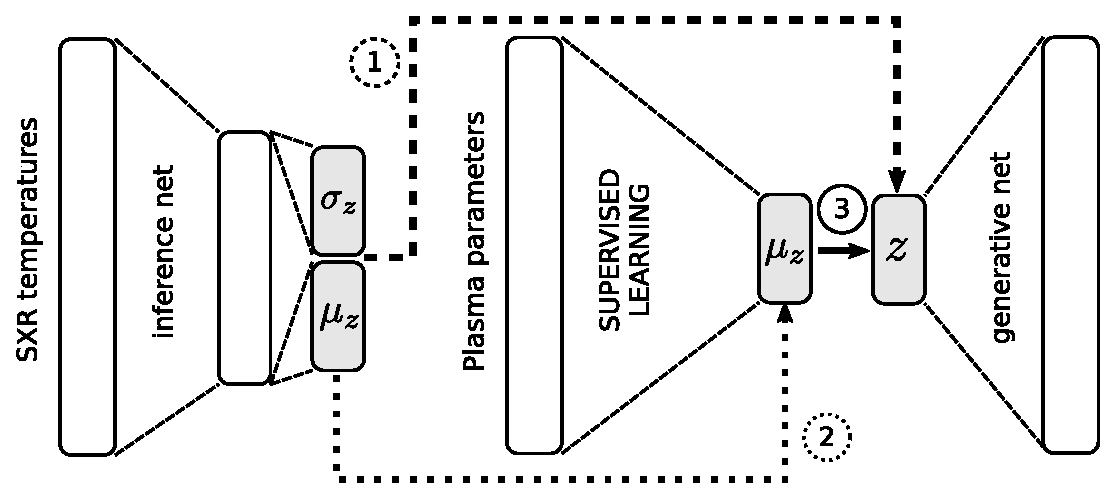
\includegraphics[height=5cm]{img/STEP12_7/SXR_from_PARAMS.eps}
    \caption{Schematic diagram of the unsupervised generative model and subsequent supervised regression that are chained to create a model able to guess the SXR profile from the sole magnetic configuration and standard plasma parameters ($Ip$,$F$,$\Theta$,$Ns$). }
    \label{fig:SXR_from_param}
\end{figure}
where a standard \acs{VAE} model is trained in advance connecting an inference network to a generative network and comparing inputs with results ( dashed path marked as step 1 ), then once the training is finished the same model is used to produce labels of a supervised neural network that learns to match external parameters to latent space determinations ( dotted path marked as step 2 ). Finally the last trained network is used to feed the \acs{VAE} decoder to complete the chain passing from parameters to profile smoothly (step 3).

The beauty of the \TF framework come again to ease the syntax: once we have a vae model trained the dataset map function can be used to generate labels online given the feature taken from dataset; in this way a couple (feature, label) can be created to be used for the supervised training.
An example of this use of network to preconditioning dataset could be the following: \\
\verb|new_ds = ds.map(lambda p,xy: (p, vae.encode(xy ,training=False))| \\
where \verb|vae| is the pre-trained model and \verb|ds| is the current dataset exposing the couple (\textit{parameters}, \textit{SXR}).
The corresponding python lines that define the model are instead the following: \\
\verb|vae = models.AEFIT5.AEFIT5(latent_dim=6, feature_dim=30, dprate=0.1,|\\
\verb|                           beta=0., scale=2, geometry=[20,20,10,10])|\\

Some example of generated profiles have been shown in~\Figure{\ref{fig:step_12_7_rec}}; where the three curves represents the related profiles from the generator output. The dashed curve in blue is a plot of the real acquired temperature data that have been cleaned up with a preliminary passage through a recovery autoencoder. The orange cross markers (+) represent the decoded output of the latent space point that corresponds to the input feature (i.e. the blue curve), and it will become the label of the supervised training. Finally the output of the second encoder - the supervised trained network - is passed through the same decoder, generating the output profile with green markers ($\times$), of the guessed temperature.
\begin{figure}
    \centering
    \subfigure{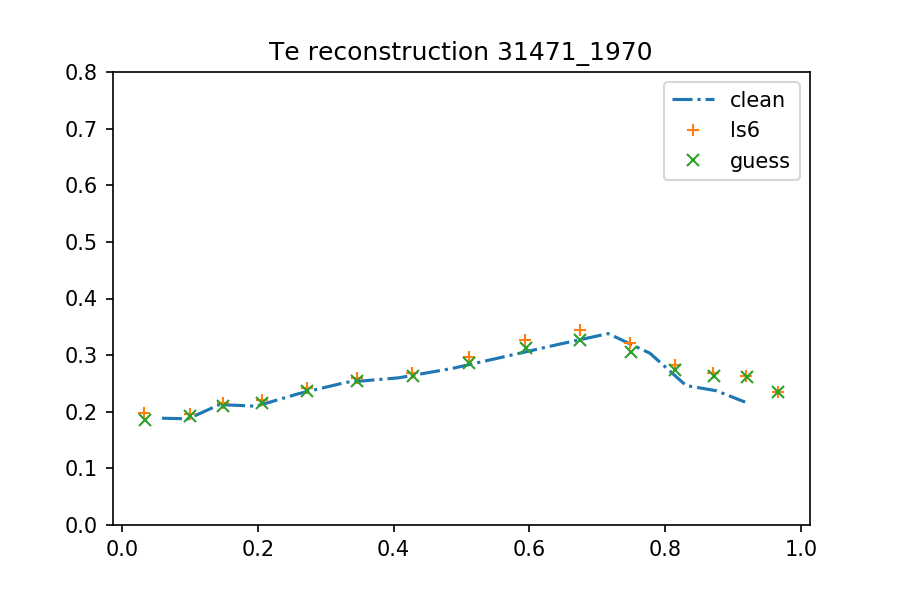
\includegraphics[height=4.8cm]{img/STEP12_7/Te_rec_215.png} }
%   \subfigure{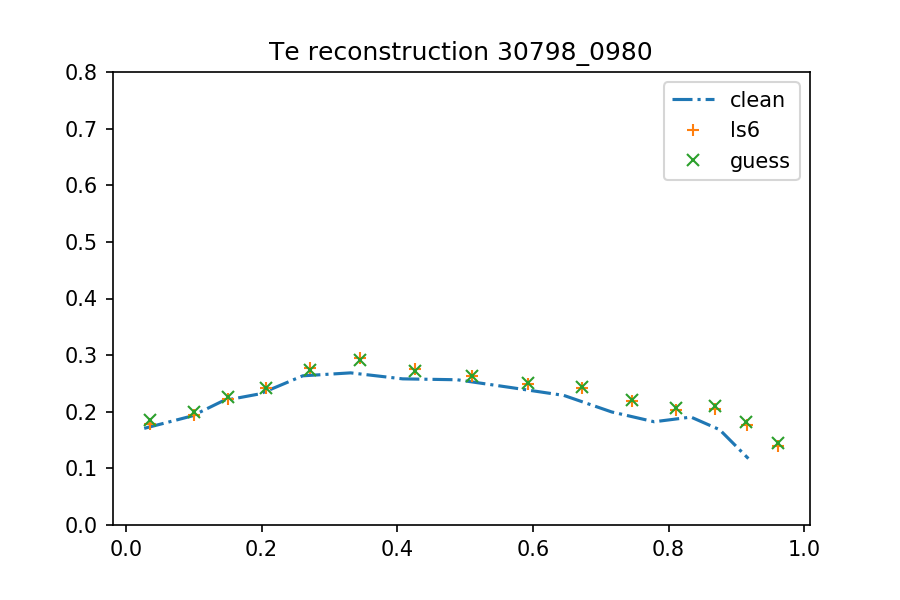
\includegraphics[height=4.8cm]{img/STEP12_7/Te_rec_219.png} }
    \subfigure{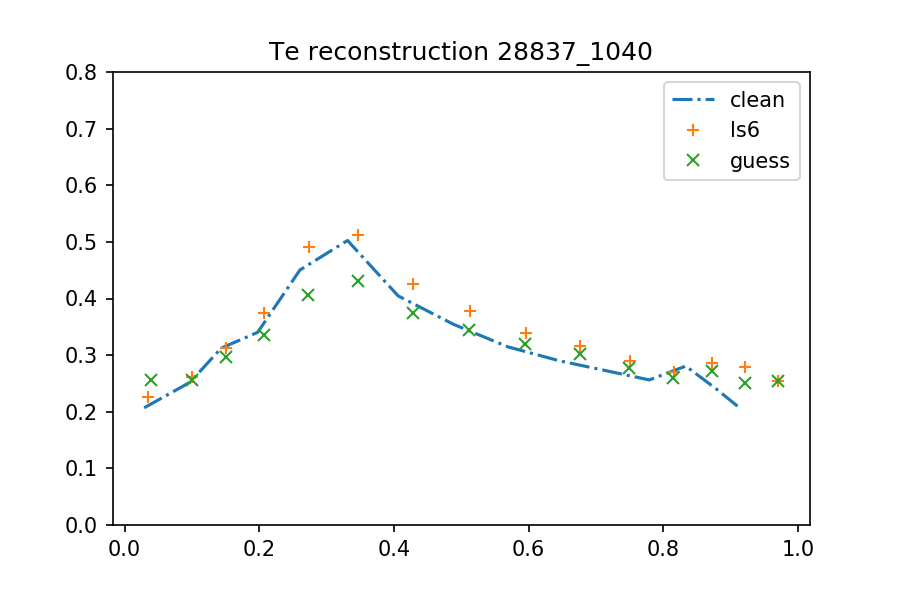
\includegraphics[height=4.8cm]{img/STEP12_7/Te_rec_229.png} }
    \subfigure{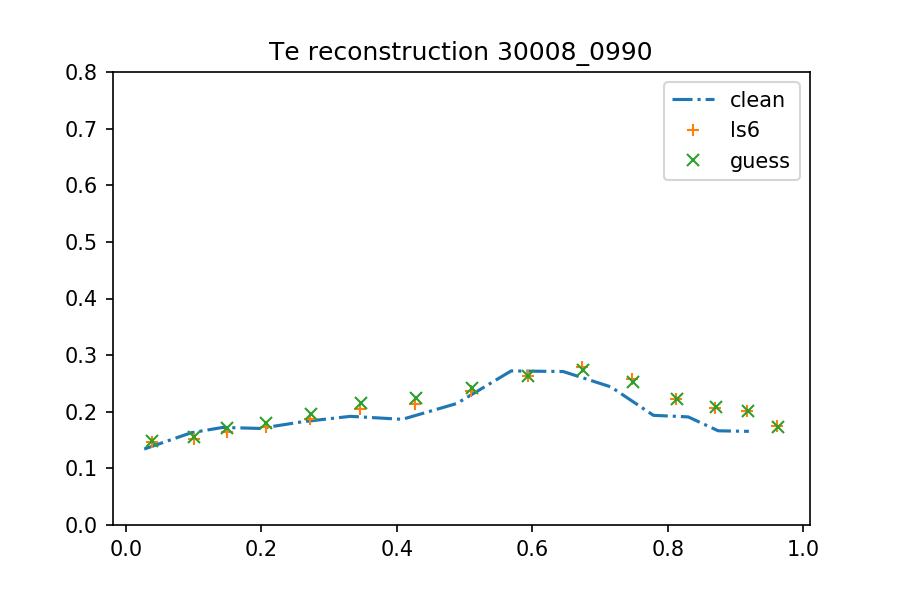
\includegraphics[height=4.8cm]{img/STEP12_7/Te_rec_232.png} }
%   \subfigure{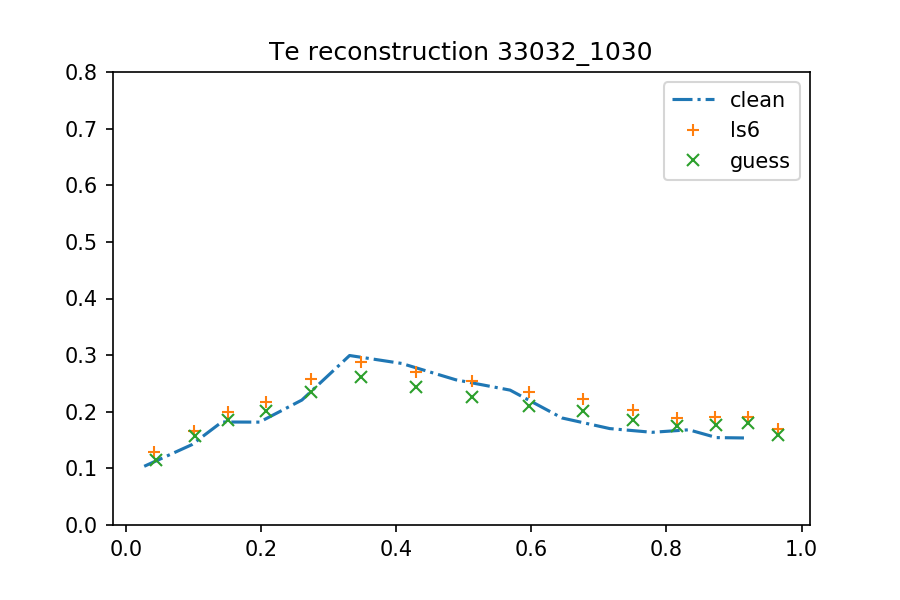
\includegraphics[height=4.8cm]{img/STEP12_7/Te_rec_243.png} }
    \subfigure{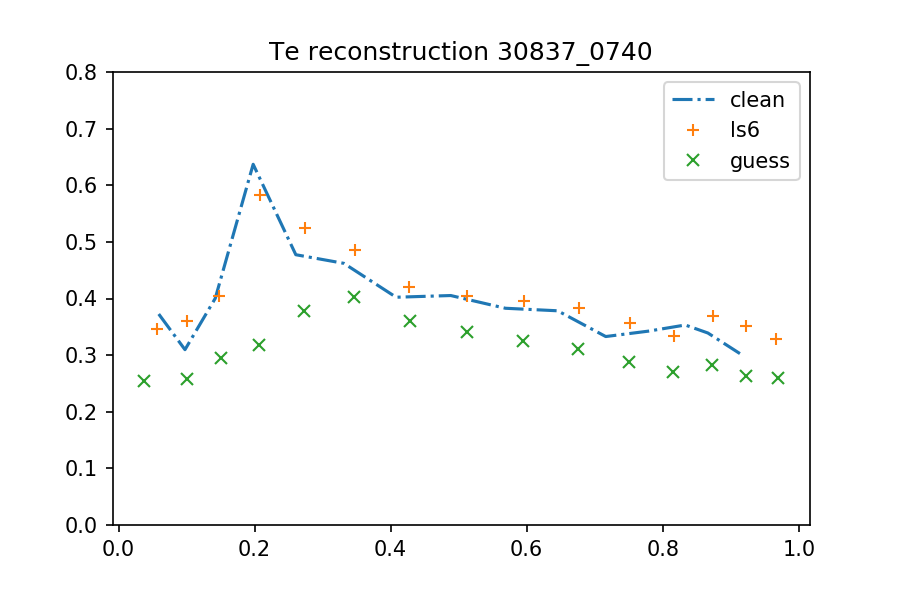
\includegraphics[height=4.8cm]{img/STEP12_7/Te_rec_213.png} }
    \caption{ Training 500 epochs - STEP 12.7 mse, slightly overfitted but validation not diverging }
    \label{fig:step_12_7_rec}
\end{figure}
The direct comparison among these plotted examples shows that the network is actually able to identify the overall shape of the profile, and it is also successfully matching the phase of the dominant perturbation. 

%   ____                                _             
%  / ___|___  _ __ ___  _ __   ___  ___(_)_ __   __ _ 
% | |   / _ \| '_ ` _ \| '_ \ / _ \/ __| | '_ \ / _` |
% | |__| (_) | | | | | | |_) | (_) \__ \ | | | | (_| |
%  \____\___/|_| |_| |_| .__/ \___/|___/_|_| |_|\__, |
%                      |_|                      |___/ 

\section{Composing Autoencoders}

Until now the only data that has been accounted is either the temperature profile or the plasma parameters, and each of them has been considered by itself. The neural network approach shown that it is possible to learn how to transfer the common hidden factors that drive experimental outcomes from one diagnostic to another, and in particular a latent space embedding helps to match such information.
However, aiming at finding a comprehensive representation of the system, a more favourable approach would be to integrate those information together in a unique latent "state" space representation.

The actual idea that follows the intuition of a hierarchical subdivision of the complete data inputs in sub domains, each represented by means of embedded manifold, has been realized as a chain of nested autoencoders. This is actually as simple as a new class method that created a nested internal structure from a input list of other autoencoders; this has been named \textit{composing}, and a schema of the built topology is proposed in~\Figure{\ref{fig:VAE_compose}}.
The simple code has been reported in~\Code{\ref{code:VAE_compose}} for the \TF implementation.
%
\begin{lstlisting}[language=Python, caption=Internal VAE method to create the composed network topology, label=code:VAE_compose]
def compose(self, autoencoders):
    from itertools import chain 
    vaes = autoencoders

    i_inputs   = list(chain.from_iterable([ get_inference_inputs(m) for m in vaes ]))
    i_outputs  = list(chain.from_iterable([ get_inference_outputs(m) for m in vaes ]))
    inf_append = tf.keras.layers.Concatenate()( i_outputs )
    self.inference_net = tf.keras.Model(i_inputs, 
                                        self._model.inference_net(inf_append), 
                                        name='compose_inference_net')
    
    g_outputs = list(chain.from_iterable([ get_generative_outputs(m) for m in vaes ]))
    g_inputs  = list(chain.from_iterable([ get_generative_inputs(m) for m in vaes ]))
    gen_append = tf.keras.Model(g_inputs, g_outputs)
    
    splits_z = [ i.shape[1] for i in g_inputs ]

    dout  = self._model.generative_net.output
    gen_split = tf.keras.layers.Lambda(lambda x: tf.split(x,num_or_size_splits=splits_z, axis=1)
                                      ) (dout)        
    self.generative_net = tf.keras.Model(self._model.generative_net.inputs, 
                                         gen_append(gen_split), 
                                         name='compose_generative_net')        
    
    i_inputs_shapes = [ get_inference_inputshape(m) for m in vaes ]

    self.inference_net.build(input_shape=i_inputs_shapes)
    self.generative_net.build(input_shape=self._model.generative_net.input_shape)
    self.output_names = [ m.generative_net.output_names for m in vaes ]

    self._mkids = vaes
    return self
\end{lstlisting}
The~\Figure{\ref{fig:VAE_compose}} shows how encoders can be connected together: each component is not directly modified but the defined internal layers are referenced inside the new structure. In this way all the autoencoders can live independently from the composition, and can be either trained one by one separately or in the composed hierarchy. This seems a complication of the overall structure that could have been managed in a single big model; however it turns to be in facts on the opposite a simplification, where a pre-training can be done independently and the training of each component, or the nested composing structure, can be interactively activated or deactivated.
Moreover, as already discussed, the use of embedded spaces appears to be not only a way to integrate heterogeneous data together, but also to create a compact representation that can be faster to train and modular. Where the term modular in this context means the possibility to localize part of computation close to the target diagnostic.
\begin{figure}
    \centering
    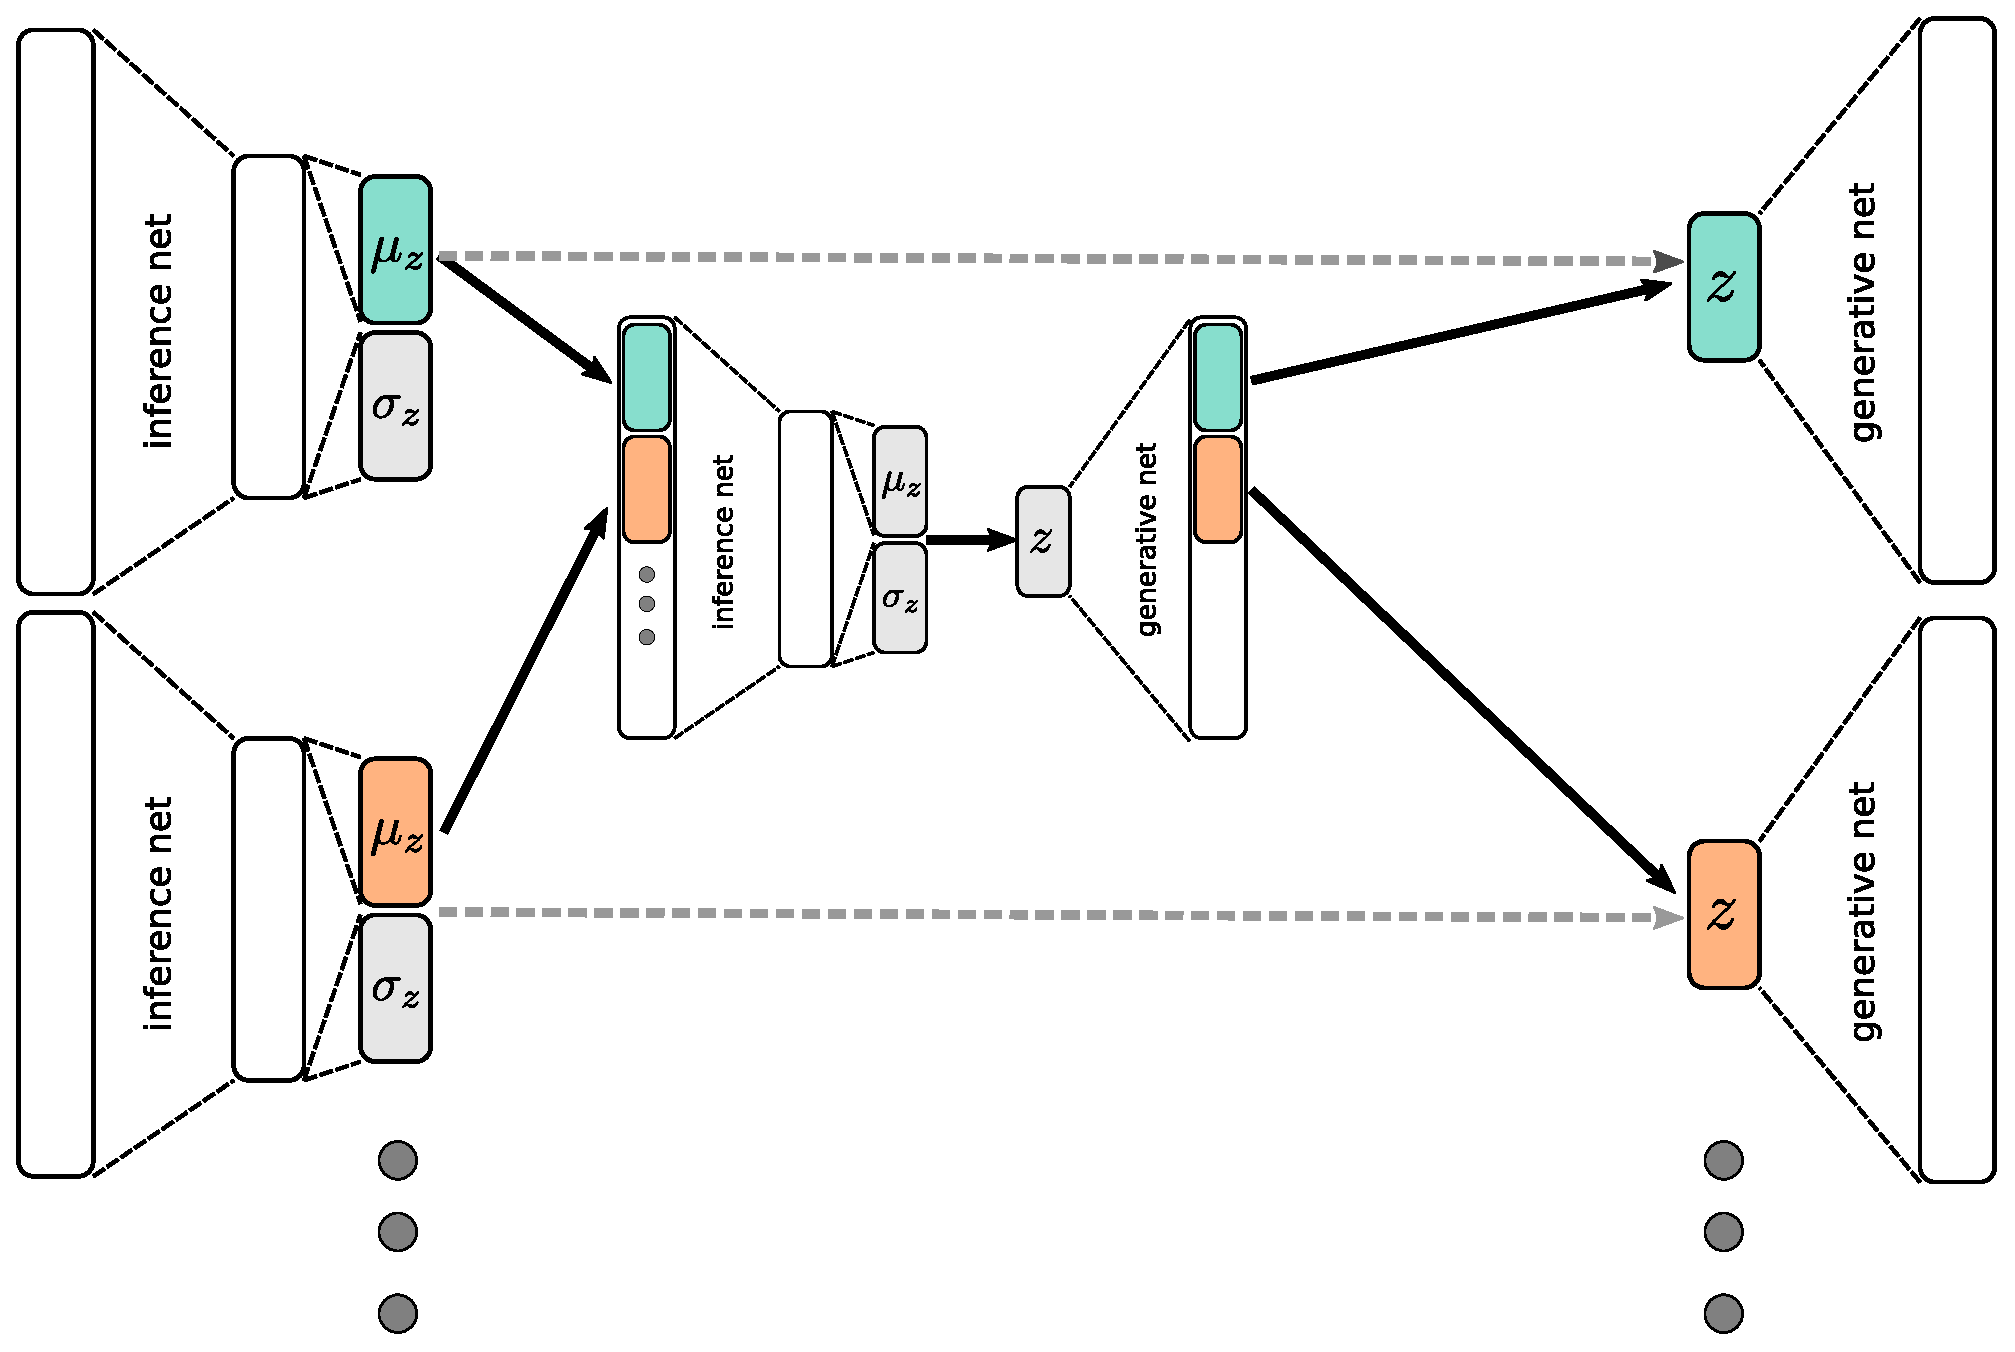
\includegraphics[height=6cm]{img/3_ML/VAE_COMPOSE.eps}
    \caption{Schematic view of the VAE composition algorithm; the first set of autoencoder can be independently trained following the dashed arrow, while the latent space variable are at the same time fed to a nested autoencoder that uses a mix of information coming from the from different representations. }
    \label{fig:VAE_compose}
\end{figure}
%
In the presented schema, and implementation, all the components are composed in the same level; one could argue that in this way the different inputs could be treated with the same "importance", however the complete network itself - once the overfiting and underfitting have been paced - tends to build paths that assign the best weights to each parameter, specially if the correct regularization and sparsification has been applied. In addition all the separate \acs{VAE} components do not need to share the same structure, givin a chance to increase or reduce the with and height (aka, the layer sizes and network depth) of each component, adding also custom network or data regularizers.

In this case we does not have a concrete output, because the actual target of this high level representation is to find a possible set of hyperparamters of the overall composition of diagnostics. However looking at the complete composed autoencoder with its property of missing data recovering, the intimate meaning of this mechanism rise up suggesting that the complex nonlinear internal relation that have been created collaborate together to describe the experiment. There can be a sufficient input set to create the missing parameter or not, either way the output is the best match of the recorded situation along the overall already seen behavior of the observed system.
For example, if two composed autoencoders would be represented by the SXR temperatures and the magnetics, the phase of the dominant mode would enforce the temperature peak position in the profile, while the plasma current would do the same for the peak height.
